{\color{indiagreen}\subsection{Kinetična energija}}
\begin{align*}
	A &= Fs\\
	F &= ma\\
	a &= \frac{\Delta v}{t} = \frac{v_2-v_1}{t}\\
	S &= \overline{v}t = \frac{v_2-v_1}{2}t\\
	A &= m\frac{v_2-v_1}{\cancelto{}{t}}\frac{v_2-v_1}{2}t\\
	A &= \frac{m}{2}(v_2^2-v_1^2)\\
	{\color{bostonuniversityred}A} &= {\color{bostonuniversityred}\frac{mv_2^2}{2} - \frac{mv_1^2}{2}}\\
	{\color{bostonuniversityred}W_k} &= {\color{bostonuniversityred}\frac{mv^2}{2}}[J] \dots \text{kinetična energija}\\
	{\color{bostonuniversityred}A} &= {\color{bostonuniversityred}W_{k2} - W_{k1} = \Delta W_k} \text{izrek o kinetični energiji}\\
\end{align*}
$v_1$ \dots začetna hitrost\\
$v_2$ \dots končna hitrost\\
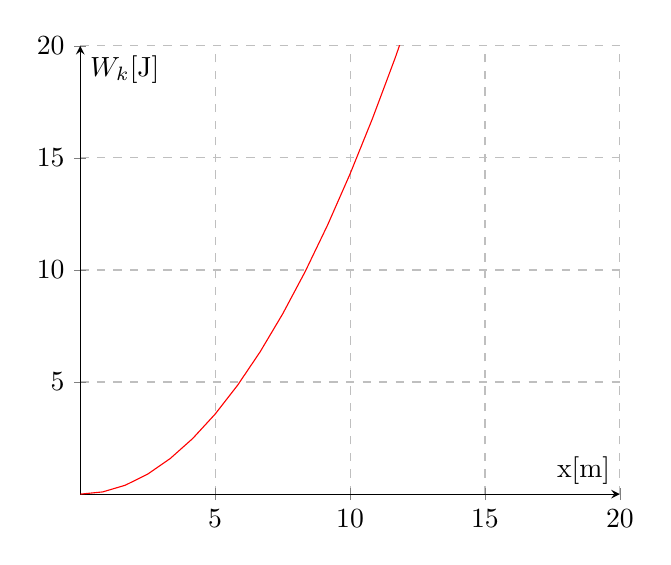
\begin{tikzpicture}
	\begin{axis}[
	    xlabel={x[m]},
	    ylabel={$W_k$[J]},
	    xmin=0, xmax=20,
	    ymin=0, ymax=20,
	    xtick={0,5,10,15,20},
	    ytick={0,5,10,15,20},
	    ymajorgrids=true,
	    xmajorgrids=true,
	    grid style=dashed,
	    axis lines=middle,
	]
	 
	\addplot[domain=0:20,red] {x^2/7};

	\end{axis}
\end{tikzpicture}